\documentclass[11pt]{article}
\usepackage[a4paper, margin=1cm]{geometry}
\usepackage[utf8]{inputenc}
\usepackage{babel}
\usepackage[spanish]{layout}
\usepackage[article]{ragged2e}
\usepackage{textcomp}
\usepackage{amsmath}
\usepackage{amssymb}
\usepackage{amsfonts}
\usepackage{proof}
\usepackage{enumerate}
\usepackage{graphicx}
\usepackage{multirow}
\usepackage{caption}
\usepackage{subcaption}

\setlength{\parindent}{0pt}

\title{
    Entrega 5 \\
    \large Sistemas Operativos II}
\author{Mellino, Natalia \and Farizano, Juan Ignacio}
\date{}

\begin{document}
\maketitle

\noindent\rule{\textwidth}{1pt}

\section*{Ejercicio 1}

Los objetivos que contradice son:

\begin{itemize} 
    \item \textbf{Ser predecible:} Un mismo trabajo debe tomar aproximadamente la misma
          cantidad de tiempo en completarse independientemente de la carga
          del sistema.

    \item \textbf{Equilibrar el uso de recursos:} Favorecer a los procesos que empleen recur-
           sos subutilizados, penalizar a los que peleen por un recurso sobreuti-
           lizado causando contención en el sistema.

    \item \textbf{Favorecer el uso esperado del sistema:} en un sistema con usuarios interactivos
          se maximiza la prioridad de los procesos que sirvan a solicitudes iniciadas por éste.

    \item \textbf{Dar preferencia a los procesos que podrían causar bloqueo:} si un proceso de 
          baja prioridad está usando un recurso que más procesos están esperando, favorecer
          que éste termine más rápido.

    \item \textbf{Favorecer los procesos con un comportamiento deseable:} penalizar los procesos
          que causa mucha demora porque degrada el rendimiento global del sistema.
\end{itemize}

Estos objetivos se contradicen por el hecho de que se refieren a favorecer a cierto
proceso de una forma u otra. El CFS tiene la idea de CPU multitarea ideal y 
precisa en dónde el poder de cómputo es repartido equitativamente. Esto
claramente va en contra de los objetivos mencionados arriba donde no se cumple
el principio de equidad que se plantea en CFS.

\section*{Ejercicio 2}

Similarmente al viejo O(1) scheduler, en CFS las tareas interactivas reciben un
priority bonus basado en un cálculo del tiempo promedio dormido (average sleep
time) lo cual les permite obtener un buen tiempo de CPU cuando lo necesitan.

\newpage
\section*{Ejercicio 3}
\begin{figure}[h!]
  \begin{center}
    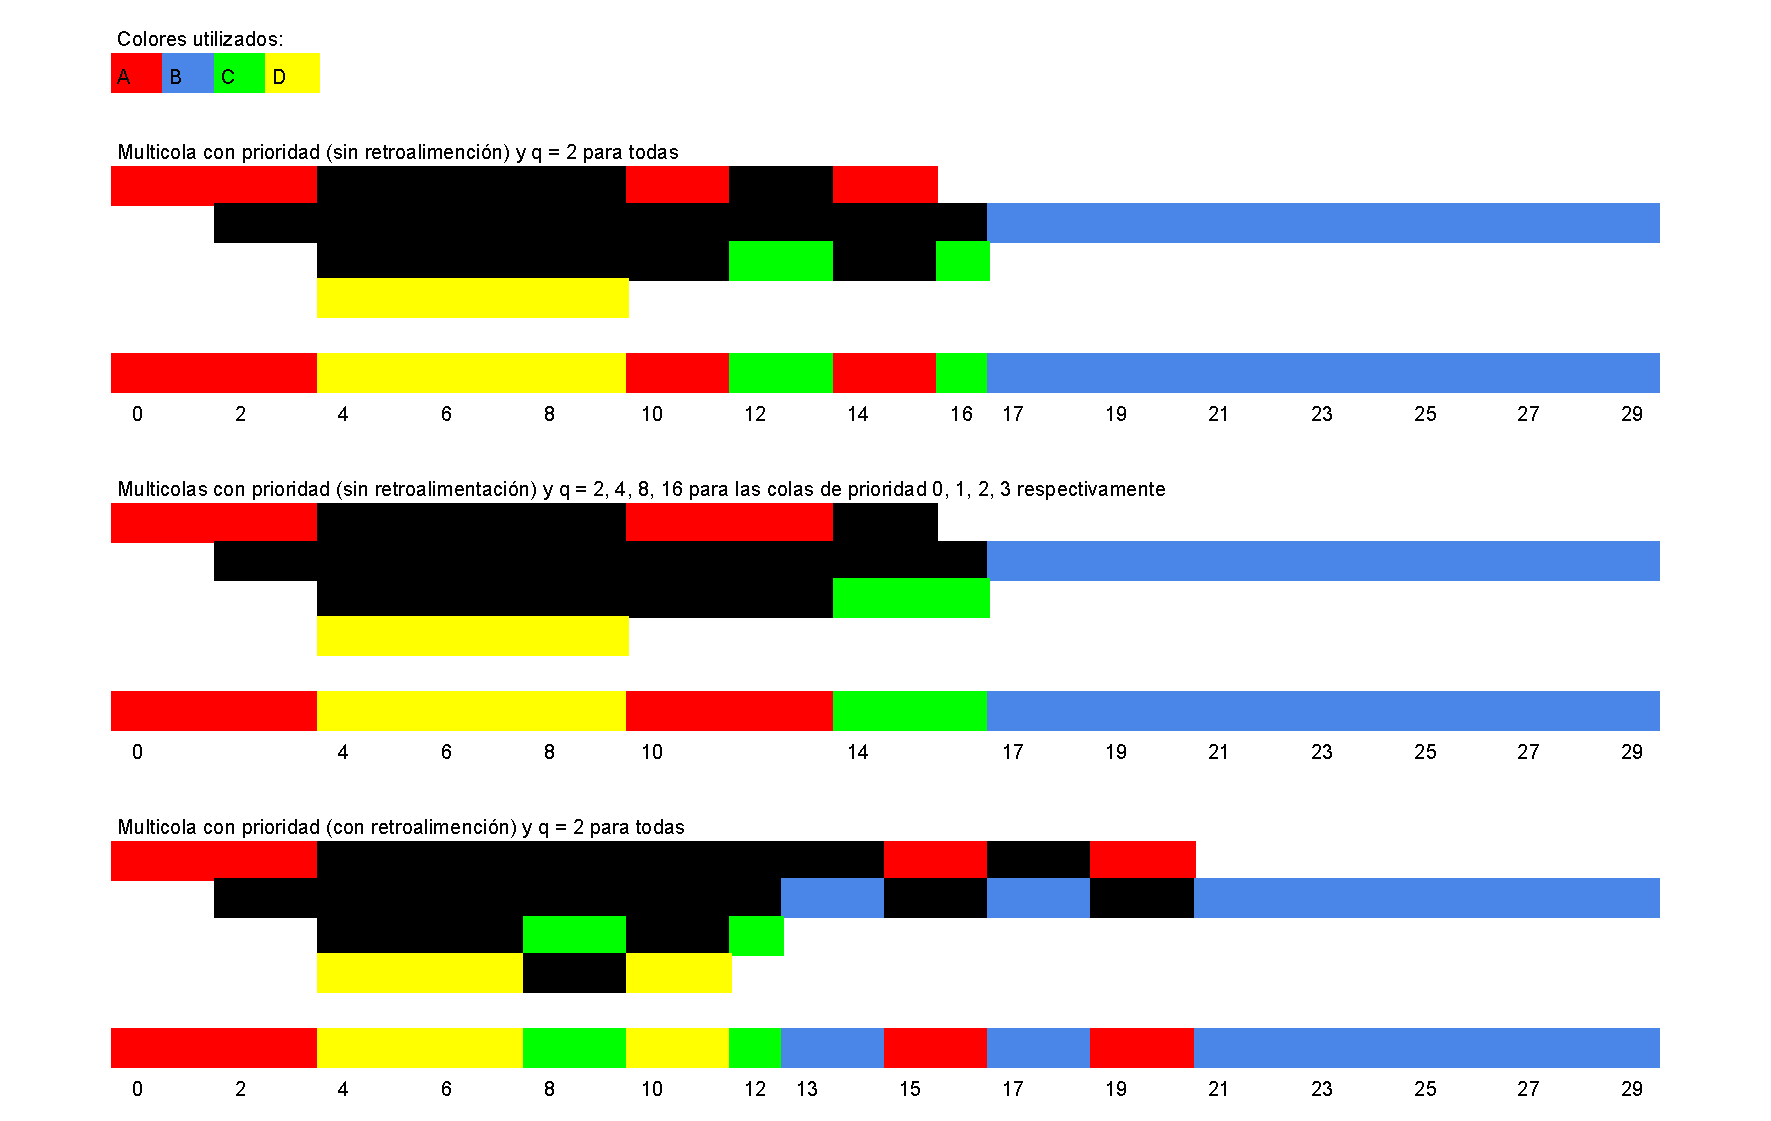
\includegraphics[width=\linewidth]{procesos.pdf}
  \end{center}
\end{figure}

\begin{table}[h!]
\begin{center}
      \begin{tabular}{|c|c|c|c|c|c|c|c|c|}
          \hline
          Proceso & Prioridad & Llegada & $t$ & Inicio & Fin & T & E & P \\
          \hline
          A & 1 & 0 & 8 & 0 & 10 & 10 & 2 & 1.25 \\
          \hline
          B & 2 & 2 & 13 & 17 & 30 & 13 & 0 & 1 \\
          \hline
          C & 1 & 4 & 3 & 14 & 17 & 3 & 0 & 1 \\
          \hline
          D & 0 & 4 & 6 & 6 & 14 & 8 & 2 & 1.3 \\
          \hline
      \end{tabular}
      \caption{Análisis despachador punto a)}
\end{center}
\end{table}

\begin{table}[h!]
\begin{center}
      \begin{tabular}{|c|c|c|c|c|c|c|c|c|}
            \hline
            Proceso & Prioridad & Llegada & $t$ & Inicio & Fin & T & E & P \\
            \hline
            A & 1 & 0 & 8 & 0 & 10 & 10 & 2 & 1.25 \\
            \hline
            B & 2 & 2 & 13 & 17 & 30 & 13 & 0 & 1 \\
            \hline
            C & 1 & 4 & 3 & 14 & 17 & 3 & 0 & 1 \\
            \hline
            D & 0 & 4 & 6 & 6 & 14 & 8 & 2 & 1.3 \\
            \hline
        \end{tabular}
      \caption{Análisis despachador punto b)}
\end{center}
\end{table}

\begin{table}[h!]
\begin{center}
      \begin{tabular}{|c|c|c|c|c|c|c|c|c|}
          \hline
          Proceso & Prioridad & Llegada & $t$ & Inicio & Fin & T & E & P \\
          \hline
          A & 1 & 0 & 8 & 0 & 16 & 16 & 8 & 2 \\
          \hline
          B & 2 & 2 & 13 & 17 & 30 & 13 & 0 & 1 \\
          \hline
          C & 1 & 4 & 3 & 10 & 17 & 7 & 4 & 2.3 \\
          \hline
          D & 0 & 4 & 6 & 4 & 14 & 10 & 4 & 1.6 \\
          \hline
      \end{tabular}
      \caption{Análisis despachador punto c)}
\end{center}
\end{table}

\end{document}